\documentclass[11pt]{article}
\usepackage[margin=1in]{geometry}
\usepackage{graphicx}
\usepackage{booktabs}
\usepackage[colorlinks=true,citecolor=blue,linkcolor=blue,urlcolor=blue]{hyperref}

\title{A Linear-Fit Micro-Experiment as a Research OS Smoke Test}
\author{}
\date{\today}

\begin{document}
\maketitle

\begin{abstract}
This note is the worked example for the AI-Human Research OS. It walks one idea
through the full loop — OKF idea concept, project instantiation from the template,
a runnable experiment, a generated figure, and a compiled PDF — with every
number traceable to code in \texttt{Code/}.
\end{abstract}

\section{Setup}
We generate $N=50$ points from $y = 2x + 1 + \varepsilon$ with
$\varepsilon \sim \mathcal{N}(0, 0.5^2)$ and a fixed seed (42), then fit a
degree-1 polynomial by least squares (\texttt{numpy.polyfit}). The script is
\texttt{Code/fit\_line.py}; run it with \texttt{uv run python fit\_line.py}.
The citation pipeline is exercised with a real reference fetched from the arXiv
API~\cite{vaswani2017attention}.

\section{Result}
The fit recovers the generating parameters: fitted slope $2.0452$ (true $2.0$),
fitted intercept $0.9325$ (true $1.0$), $\mathrm{MSE}=0.1402$
(script output, 2026-06-12). Figure~\ref{fig:fit} shows the data and the
fitted line.

\begin{figure}[h]\centering
  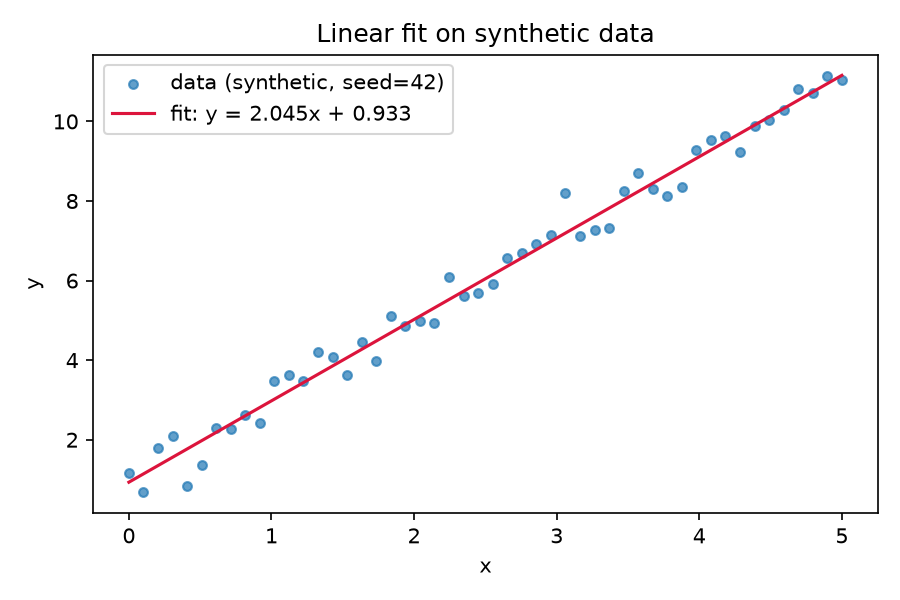
\includegraphics[width=.8\linewidth]{../Figs/linear_fit.png}
  \caption{Synthetic data and least-squares linear fit (seed 42).}
  \label{fig:fit}
\end{figure}

% Build from the project root: cd paper && latexmk -pdf -bibfudge- -interaction=nonstopmode -outdir=../build main.tex
% (-bibfudge- makes bibtex run from paper/, so the relative path below
%  resolves against the paper/ directory even when output goes to ../build.)
% Bibliography: shared store at the repository root (project sits at root level).
\bibliographystyle{plain}
\bibliography{../../References/refs}

\end{document}
